\documentclass[twocolumn]{article}
\usepackage[table]{xcolor}
\usepackage{listings}
\usepackage{amsmath}
\usepackage{fullpage}
\usepackage{tabularx}
\usepackage{graphicx}
\usepackage{caption}
\usepackage{subcaption}
\usepackage{tikz}
\usetikzlibrary{shapes.geometric, arrows}
\usepackage{cite}
\usepackage{hyperref}
\usepackage{float}
%\usepackage{authblk}

\begin{document}
\lstset{language=python, tabsize=4}
\title{Collaborative rating prediction with artificial neural networks}

%\author[1]{Yuchen Hou \thanks{yuchen.hou@wsu.edu}}
%\author[1]{Lawrence B. Holder \thanks{holder@wsu.edu}}
%\affil[1]{School of Electrical Engineering and Computer Science\\
%	Washington State University\\
%	Pullman, WA 99164}
\maketitle

\begin{abstract}
	The applications of neural networks are very successful in various domains 
	including image recognition, speech recognition and natural language 
	processing.
	However, its application in graph mining is not well studied.
	Here we present node mapping, a technique created for link attribute 
	prediction powered by neural networks.
	This technique extracts knowledge of nodes from known links and uses this 
	knowledge to predict unknown links.
	We demonstrate the power of this technique in a famous social network 
	application scenario: recommender systems.
	Our experiments show that the node mapping technique can provide a new
	recommendation solution that outperforms collaborative filtering 
	technique by up to 17\% in terms of prediction accuracy.
	We anticipate this new technique to provide effective solutions to more 
	prediction tasks in different graph applications.
\end{abstract}

\section{Introduction}
The expression deep learning existed as early as 1986 in machine learning 
community \cite{dechter1986learning}, though not so well known for many years.
But now, deep learning techniques using neural network models are rapidly 
gaining traction in many application domains 
such as:
\begin{itemize}
	\item speech recognition \cite{hannun2014deep}
	\item image recognition \cite{simonyan2014very}
	\item natural language processing \cite{yao2013recurrent}
	\item graph mining \cite{grovernode2vec}
	\item drug discovery \cite{dahl2014multi}
	\item recommendation systems \cite{barkan2016item2vec}
\end{itemize}
Two reasons for its adoptions in these domains are its higher prediction 
accuracy and less engineering compared to other machine learning techniques.
Among these domains, research in recommendation systems has been very active  
due to its extremely high value in industries such as search, e-commerce, 
travel and social \cite{buettner2016predicting}.
Recommendation systems are classified into two groups according to the way they 
extract information about items: content based filtering and collaborative 
filtering \cite{ricci2011introduction}.
Collaborative filtering extract information from the relations between users 
and items, while content based filtering extracts information from the contents 
of items.
Collaborative filtering has multiple forms including producing a list of items 
a user would like, and predicting the ratings a user would give to a list of 
items \cite{su2009survey}.
The focus of this paper is the rating prediction form of collaborative 
filtering, which we call collaborative rating prediction.
The contribution of this paper is a deep learning application in 
collaborative rating prediction, which we believe is the first of its kind.

\section{Related work}
In this section,
we review a few existing deep learning applications in both content based 
filtering and collaborative filtering.
We also clarify how our work differs from these related work.

\subsection{Content based applications}
Applications in this group extract information of an item from its content, 
i.e., the input of the neural network is a vector produced from the item's 
content (e.g., the audio of the song, the text of an article):
\begin{itemize}
	\item One example is a music recommendation system \cite{van2013deep}. 
	It is a tag prediction system implemented with a convolutional neural net: 
	the input is the spectrogram vector of the audio of a song, and the output 
	is the set of tags of the song (e.g., genre, instrumentation, tempo, mood).
	\item Another example is a multi-view recommendation system 
	\cite{elkahky2015multi}. 
	It is a rating prediction system implemented with a fully connected neural 
	net: the input is the letter tri-gram vector of the text description of a 
	news article, app or movie, and the output is the rating.
\end{itemize}
Obviously, these applications are very similar to image recognition and speech 
recognition.
Our work differs from them in that our technique does not access the contents 
of items.

\subsection{Collaborative applications}
Applications in this group extract information of an item from its relations 
with other items, and the input of the neural net is a vector learned by the 
neural net itself from the relations between items.
All these applications treat a list of items as a sentence of words 
(effectively reducing their problems to a natural language processing problem)  
and then apply the famous skip-gram model used in word2vec 
\cite{mikolov2013efficient}:
\begin{itemize}
	\item An item similarity prediction example is item2vec 
	\cite{barkan2016item2vec} where purchase orders (lists of items) are 
	treated as sentences.
	\item Similar examples exist in graph mining, like deep walk 
	\cite{perozzi2014deepwalk} and node2vec \cite{grovernode2vec}, where a 
	graph is sampled into walks (lists of nodes), and treated as sentences.
\end{itemize}
One drawback of these applications is that they fail to take advantage of 
the highly organized, regular and repeated structure in their relational data: 
relations between users and items (i.e., a user gives numerical rating to an 
item) and relations between nodes (i.e., a source node connects to a 
destination node though a labeled link).
This nice structure is not exploited in natural language processing because it 
does not exist (i.e., for a neural net, words can simply show up in a sequence 
from a day-to-day conversation, in many flexible and unpredictable ways, with 
little structure or regularity).
Although syntax and semantics exist in natural languages, we have not seen any 
current neural network models taking advantage of these structures.
Our work differs from the above applications in that our technique uses a 
neural net model designed to take advantage of the structure in the relational 
data and it is also able to predict a numerical attribute - the rating value.

\section{Problem}
The problem we consider in this paper is collaborative rating prediction 
problem.
In this section, we look at an example of the problem and then its definition.

\subsection{Problem example}
This is a collaborative rating prediction problem example: 
a set of 6 users give numerical ratings to a set of 3 items.
For each user, only a subset of his ratings are known; 
and we want to predict the unknown ratings.
This example is demonstrated in \autoref{tab:ratings}.
\begin{table}[h]
	\centering
	\caption{A collaborative rating prediction problem example.
		In this example, a set of 6 users give ratings to a set of 3 items: 
		for User[0], ratings to all 3 items are known; 
		for User[1], ratings to Item[1] and Item[2] are known, 
		but the rating to Item[0] is unknown; and so on.
		Every unknown rating is marked as a question mark.
		The task is to predict the unknown ratings.
	}
	\begin{tabularx}{0.5\textwidth}{ |X|c|c|c|}  \hline \rowcolor{blue!50}
		& Item[0] & Item[1] & Item[2] \\ \hline
		User[0] & 3 & 5 & 2 \\ \hline
		User[1] & ? & 5 & 2 \\ \hline
		User[2] & 4 & 4 & 5 \\ \hline
		User[3] & 2 & 4 & ? \\ \hline
		User[4] & 5 & 5 & 4 \\ \hline
		User[5] & 4 & ? & 4 \\ \hline
	\end{tabularx}
	\label{tab:ratings}
\end{table}

\subsection{Problem definition}
Formally, a collaborative rating prediction problem is defined as follows:
\begin{itemize}
	\item given: a 2-D array R[m][n], 
	where R[i][j] is the rating User[i] gives to Item[j],
	$ i \in [0, m-1] $, j $ \in [0, n-1] $, and a number of elements in Rating 
	are unknown
	\item task: predict all unknown elements in R
\end{itemize}
Moreover, we define a user as the array of ratings he gives to all items:
\begin{align*}
	User[i] = R[i]
\end{align*}

\section{Baseline solutions}
Among many algorithms to collaborative rating prediction problem,
a prevalent one is the neighborhood-based collaborative filtering algorithm 
\cite{su2009survey}.
This algorithm also has several variants,
which we will use as baseline solutions.

\subsection{Algorithm}
The neighborhood-based collaborative filtering algorithm calculates each 
unknown R[i][j] as 
follows \cite{su2009survey}:
\begin{align*}
R[i][j] = c \sum_{k = 0}^{m-1} S(i, k) R[k][j]
\end{align*}
where S(i, k) is the similarity of User[i] and User[k] to be defined by each 
variant,
unknown R[k][j]'s are omitted and c is a normalizing factor:
\begin{align*}
	c = \frac{1}{\sum_{l = 0}^{m - 1} |S(i, k)|}
\end{align*}
It is easy to understand the predicted rating User[i] gives to Item[j] as the 
sum of ratings all users give to Item[j],
weighted by how similar each user is to the target user.
The algorithm can use only a number of users with highest similarities to the 
target user in the calculation, instead of using all users.

\subsection{Variants}
Each variant of the algorithm has a unique definition of the similarity 
function of User[i] and User[k]:
\begin{itemize}
	\item The cosing similarity is defined as \cite{sarwar2000analysis}:
	\begin{align*}
		&S_{cos}(x, y) \\
		&= \frac{R[x] \cdot R[y]}{||R[x]|| \cdot ||R[y]||} \\
		&= \frac{\sum_{i \in I_{xy}}R[x][i]R[y][i]}{\sqrt{\sum_{i \in 
		I_x}R[x][i]^2} \sqrt{\sum_{i \in I_y}R[y][i]^2}}
	\end{align*}
	where $ I_{x} $ is the set of items rated by User[x],
	and $ I_{y} $ is the set of items rated by User[y], 
	and $ I_{xy} $ is the set of items rated by both User[x] and User[y]. 
	\item The Pearson correlation coefficient (PCC) similarity is defined as 
	\cite{resnick1994grouplens}:
	\begin{align*}
		&S_{PCC}(x, y) \\
		&= \frac{\sum_{i \in I_{xy}}(R[x][i] - \overline{R[x]})(R[y][i] - 
		\overline{R[y]})}{\sum_{i \in I_{xy}}(R[x][i] - \overline{R[x]})^2 
		\sum_{i 
		\in I_{xy}}(R[y][i] - \overline{R[y]})^2 }
	\end{align*}
	where $ \overline{R[x]} $ is the average rating User[x] gives to all items.
	PCC measures the linear correlation of two users.
	\item The weighted PCC (WPCC) similarity is defined as 
	\cite{herlocker1999algorithmic}:
	\begin{align*}
		S_{WPCC}(x, y) = 
		\begin{cases}
			\frac{|I_{xy}|}{T} S_{PCC}(x, y) & |I_{xy}| < T \\
			S_{PCC}(x, y) & otherwise
		\end{cases}
	\end{align*}
	where T is a threshold of number of items. 
	WPCC of two users differs from PCC only when the number of items rated by 
	both users (co-rated items) is less than the threshold. 
	When the difference occurs, less number of co-rated items results in less 
	similarity in the two users.
	\item The sigmoid PCC (SPCC) similarity is defined as 
	\cite{jamali2009trustwalker}:
	\begin{align*}
		S_{SPCC} (x, y) = \frac{S_{SPCC}(x, y)}{1 + exp(-\frac{|I_{xy}|}{2})}
	\end{align*}
	SPCC is very similar to WPCC in the sense two users have lower similarity 
	if they have a smaller number of co-rated items.
	\item The multi-level PCC (MPCC) similarity \cite{polatidis2016multi} . 
	This one is also very similar to the previous ones but much more complex, 
	so we skip its description here.
\end{itemize}

\section{Observations and approach}
Although the various applications in related work section can not solve the 
collaborative rating prediction problem,
they all have an interesting key process: vector representations of entities.
As deep learning techniques become more powerful and standardized, this key 
process seems to be the most significant part in a domain specific deep 
learning application.
In an informal way, that is like to say: in order to apply deep learning to a 
specific task, just represent the data at hand as vectors of numbers,
feed them to the neural net, and then deep learning will take care of 
everything else.

\subsection{Entities and representations}
First of all, we summarize how a neural net represents various types of 
entities in different domains with different relations, as shown in 
\autoref{tab:domains}.
It is clear that representations for all the entities are numerical arrays, 
because neural nets rely on neurons' activations and communications, which 
are both numerical.
\begin{table}[h]
	\centering
	\caption{A summary of various types of entities, their numerical
		representations and inter-entity relations in different domains:
		Images in image recognition and utterances in speech recognition can be 
		directly represented by 2D numerical arrays, 
		but their relations to other images or utterances are not commonly 
		used. 
		Words in natural languages, items in recommendation systems, and nodes 
		in graphs can be represented by vectors (1D numerical arrays) and their 
		relations to other words, items and nodes are commonly used to learn 
		these vectors.}
	\begin{tabularx}{0.5\textwidth}{|X|c|c| } \hline \rowcolor{blue!50}
		Entity & Representation & Relations \\ \hline
		image & 2D intensity array & NA \\ \hline
		utterance & 2D intensity array & NA \\ \hline
		word & word vector & co-occurrences \\ \hline
		item & item vector & co-purchases \\ \hline
		node & node vector & connections \\ \hline
	\end{tabularx}
	\label{tab:domains}
\end{table}

\subsection{Entities to vectors}
The famous word2vec technique is the first of its kind in using a neural net to 
learn to map every entity (word in this case) in a vocabulary to a vector 
without any domain knowledge \cite{mikolov2013efficient}.
The subsequent techniques item2vec and node2vec use the identical skip-gram 
model to map items and nodes to vectors.
\autoref{tab:word} shows a mapping table that maps each word ID to the word 
vector.
In a corpus, every word is described/defined only by related words in its 
contexts, by implicit relations between words in word co-occurrences.
Nonetheless, the neural net can learn from word co-occurrences and map words to 
vectors accordingly,
such that the relations between words are preserved in the word vector space 
\cite{mikolov2013distributed}.
The same arguments apply to relations between items and nodes.
\begin{table}[h]
	\centering
	\caption{Entity (word/item/node) to vector mapping table for a set of n
		entities with entity vectors of size d:
		Each entity has an ID.
		The values of vectors in this table are hypothetical.}
	\begin{tabularx}{0.5\textwidth}{|c|X|} \hline \rowcolor{blue!50}
		Entity ID & Entity (word/item/node) vector \\ \hline
		1 & [2.3, 564, -9.5 ... 3] \\ \hline
		2 & [76, -342.2, 0.3 ... 4.2] \\ \hline
		3 & [-345, -834, 0.3 ... 34] \\ \hline
		... & ... \\ \hline
		n & $ [x_1, x_2, x_3 ... x_d] $ \\ \hline
	\end{tabularx}
	\label{tab:word}
\end{table}

\subsection{Users and items to vectors}
However, the relation between a user and an item is quite different from that 
between words:
\begin{itemize}
	\item The rating a user gives to an item explicitly tells us how much the 
	user likes that item;
	the relation is very specific: one user, one item, one rating - no more, no 
	less.
	\item The co-occurrences of words [the, quick, brown, fox, jumps, over] 
	implicitly tell us these words are related but do not tell us any specific 
	relation.
\end{itemize}
This observation suggests that a neural net should be able to learn user to 
vector mapping and item to vector mapping supervised by the rating, in a more 
specific, direct and simply way than it learns word to vector mappings 
supervised by word co-occurrences.

\section{Solution}
Formally, the prediction task is, given any (user, movie) pair, predict the 
rating the user would give to the movie:
\begin{itemize}
	\item input: X = (user, movie)
	\item output: Y = rating(user, movie)
\end{itemize}

\subsection{Conceptual model}
Using the node mapping technique, we provide a new solution to recommender 
systems: 
an estimator with a neural net model called neural recommender model, shown in 
\autoref{fig:conceptural}.
\begin{figure*}[h]
	\centering
	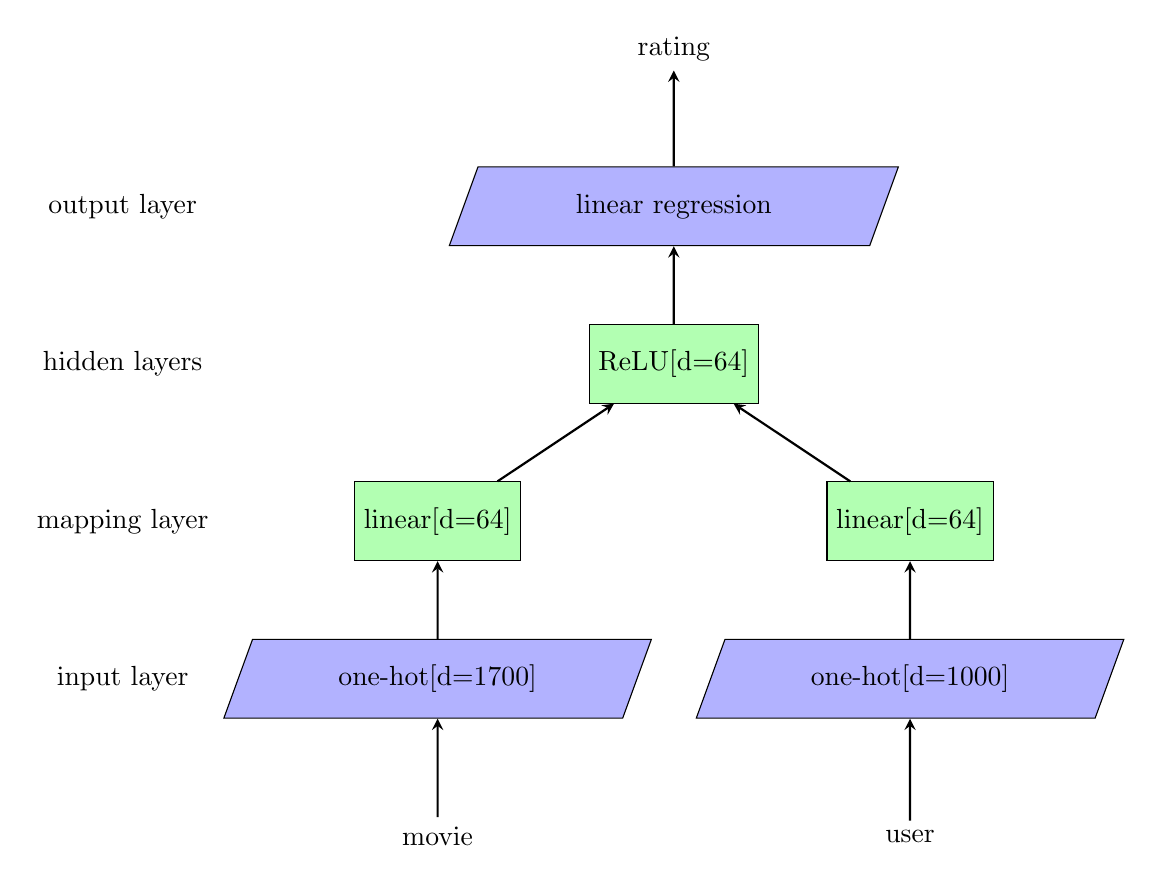
\begin{tikzpicture}[node distance=2cm]
	\tikzstyle{io} = [trapezium, trapezium left angle=70, trapezium right 
	angle=110, minimum width=1cm, minimum height=1cm, text centered, 
	draw=black, fill=blue!30]
	\tikzstyle{process} = [rectangle, minimum width=1cm, minimum height=1cm, 
	text centered, draw=black, fill=green!30]
	\tikzstyle{arrow} = [thick,->,>=stealth]
	\node (linearRegression) [io] {linear regression};
	\node (relu3) [process, below of=linearRegression] {ReLU[d=64]};
	\node (linear2) [process, below of=relu3, xshift=-3cm] {linear[d=64]};
	\node (linear1) [process, below of=relu3, xshift=3cm] {linear[d=64]};
	\node (oneHot2) [io, below of=linear1] {one-hot[d=1000]};
	\node (oneHot1) [io, below of=linear2] {one-hot[d=1700]};
	\node (rating) [above of=linearRegression] {rating};
	\node (output) [left of=linearRegression, xshift=-5cm] {output layer};
	\node (hidden1) [below of=output] {hidden layers};
	\node (mapping) [below of=hidden1] {mapping layer};
	\node (input) [below of=mapping] {input layer};
	\node (movie) [below of=oneHot1] {movie};
	\node (user) [below of=oneHot2] {user};
	\draw [arrow] (movie) -- (oneHot1);
	\draw [arrow] (user) -- (oneHot2);
	\draw [arrow] (oneHot2) -- (linear1);
	\draw [arrow] (oneHot1) -- (linear2);
	\draw [arrow] (linear1) -- (relu3);
	\draw [arrow] (linear2) -- (relu3);
	\draw [arrow] (relu3) -- (linearRegression);
	\draw [arrow] (linearRegression) -- (rating);
	\end{tikzpicture}
	\caption{The conceptual neural recommender model for a dataset with 1700 
	movies and 1000 users:
	The d in the bracket refers to dimension, the layer's size (number of 
	units in the layer).
	We keep all layers the same size for simplicity, although layers of 
	different sizes may produce better results.
	The text before the bracket refers to the activation function of the 
	units in the layer (except for one-hot, which refers to the activations 
	in the input layer).
	Only layers and their connections are shown, while the units in each 
	layer and their connections are not shown.}
	\label{fig:conceptural}
\end{figure*}
The model contains the following layers:
\begin{itemize}
	\item an input layer with one-hot activations: it has 1 channel for movies 
	and 1 channel for users;
	this layer is directly activated by the testing program (e.g., to feed the 
	1200th movie, the testing program sets 1 at the 1200th unit and 0 at other 	
	units in the movie channel);
	\item a mapping layer with linear units: it has 2 channels to map each 
	movie and each user to a vector;
	the activations of these 2 channels form the 2 node vectors (i.e., the 
	movie vector and the user vector);
	it is the most critical layer as it gradually learns to map every node to 
	the correct vector during training;
	\item several fully connected hidden layers (1 layer is shown in the figure;
	multiple numbers of layers and layer sizes are considered in the 
	experiments) of ReLU (rectified linear units):
	they have non-linear activation functions to give the model sufficient 
	complexity;
	they learn to process node vectors and produce more abstract 
	rating-relevant information;
	\item an output layer with a linear regression unit: it learns to predict 
	the rating based on processed information;
\end{itemize}
We fully take into account the characteristics of social networks when 
designing this model.
In a social network, user activities - not user profiles - provide the most 
information about users, so we design the model to learn node vectors 
supervised by link attributes.
We have considered alternative models, but we find them hard to scale.
For example, we can represent a user as the vector of movie ratings he has 
given, 
but this approach will not scale if we have an increasing number of movies.
For example, a new user will require an update to the network topology (at 
least at the input layer) and retraining.

\subsection{Actual model}
In practice, the model uses more efficient mapping tables instead of a 
one-hot input layer to handle a graph with increasing number of nodes.
\autoref{fig:actural} shows the actual model with two modifications from the 
conceptual model:
\begin{itemize}
	\item The input layer is replaced by 2 mapping tables: 1 for movie nodes 
	and 1 for user nodes;
	their inputs are node IDs and their outputs are node vectors, just like the 
	word to vector mapping table referenced in \autoref{tab:word}
	\item The mapping layer is replaced by a 2-channel input layer: it is 
	directly activated by the outputs of the mapping tables
\end{itemize}
\begin{figure*}[h]
	\centering
	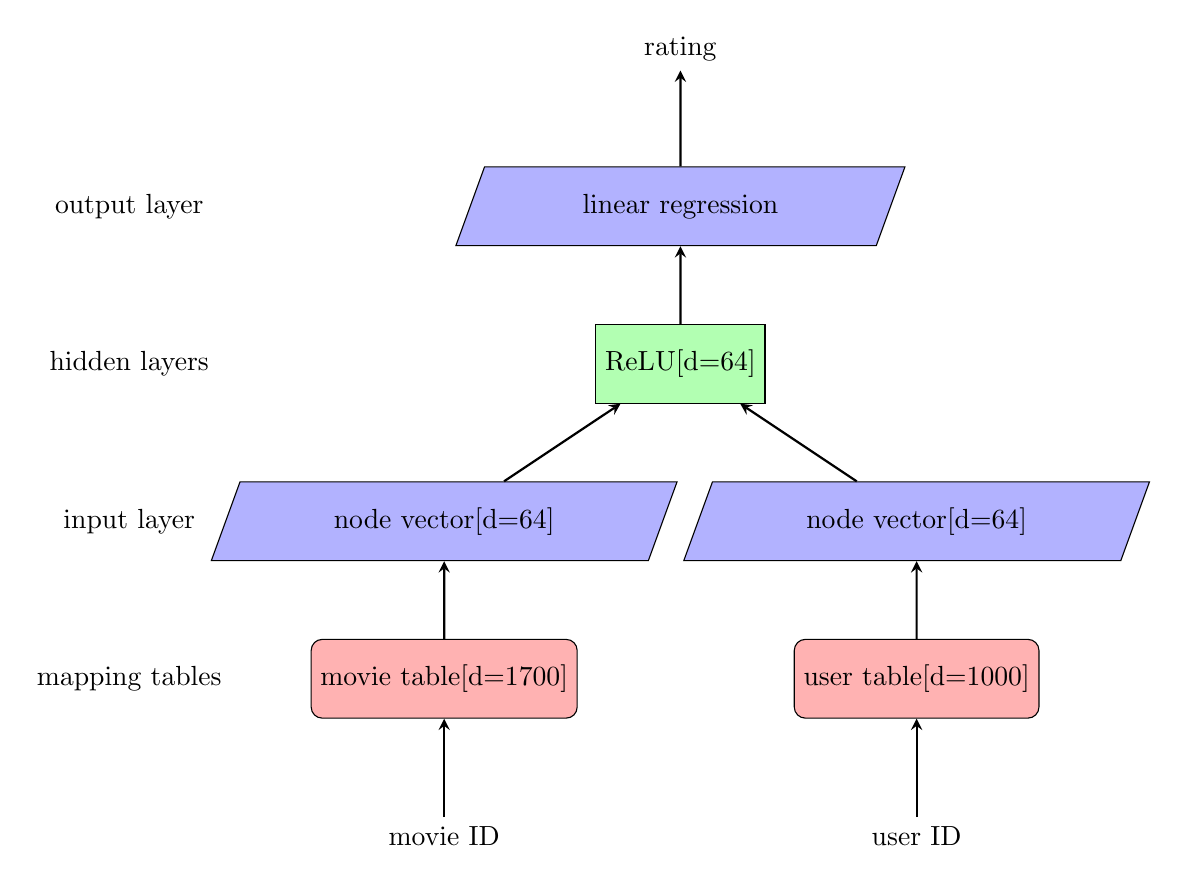
\begin{tikzpicture}[node distance=2cm]
	\tikzstyle{io} = [trapezium, trapezium left angle=70, trapezium right 
	angle=110, minimum width=1cm, minimum height=1cm, text centered, 
	draw=black, fill=blue!30]
	\tikzstyle{startstop} = [rectangle, rounded corners, minimum width=1cm, 
	minimum height=1cm, text centered, draw=black, fill=red!30]
	\tikzstyle{process} = [rectangle, minimum width=1cm, minimum height=1cm, 
	text centered, draw=black, fill=green!30]
	\tikzstyle{arrow} = [thick,->,>=stealth]
	\node (linearRegression) [io] {linear regression};
	\node (relu3) [process, below of=linearRegression] {ReLU[d=64]};
	\node (linear2) [io, below of=relu3, xshift=-3cm] {node vector[d=64]};
	\node (linear1) [io, below of=relu3, xshift=3cm] {node vector[d=64]};
	\node (oneHot2) [startstop, below of=linear1] {user table[d=1000]};
	\node (oneHot1) [startstop, below of=linear2] {movie table[d=1700]};
	\node (rating) [above of=linearRegression] {rating};
	\node (output) [left of=linearRegression, xshift=-5cm] {output layer};
	\node (hidden1) [below of=output] {hidden layers};
	\node (input) [below of=hidden1] {input layer};
	\node (mapping) [below of=input] {mapping tables};
	\node (movie) [below of=oneHot1] {movie ID};
	\node (user) [below of=oneHot2] {user ID};
	\draw [arrow] (movie) -- (oneHot1);
	\draw [arrow] (user) -- (oneHot2);
	\draw [arrow] (oneHot2) -- (linear1);
	\draw [arrow] (oneHot1) -- (linear2);
	\draw [arrow] (linear1) -- (relu3);
	\draw [arrow] (linear2) -- (relu3);
	\draw [arrow] (relu3) -- (linearRegression);
	\draw [arrow] (linearRegression) -- (rating);
	\end{tikzpicture}
	\caption{The actual model with two modifications:
		We factor the node to vector mapping process out of the neural net into 
		2 node to vector mapping tables.
		We feed every node (a movie or user) to the estimator by feeding the 
		node ID.
		During learning, the estimator updates the vectors in the tables the 
		same way it updates weights in the conceptual model.}
	\label{fig:actural}
\end{figure*}

\subsection{Learning techniques}
The estimator uses the above neural net model and a number of popular learning 
techniques:
\begin{itemize}
	\item backpropagation: propagation of the error gradients from output layer 
	back to each earlier layer \cite{rumelhart1988learning}
	\item SGD (stochastic gradient descent): the optimization that minimizes 
	the error (descending against the error gradient in weight space) for a 
	random sample in each step \cite{lecun2012efficient}
	\item mini-batch: the modification to SGD to accelerate and smooth the 
	descent by minimizing the error for a small random portion of samples in 
	each step \cite{mairal2010online}
	\item dropout (specified by keep probability): the technique to reduce unit 
	co-adaptation by temporarily dropping out a random portion of units in each 
	step \cite{srivastava2014dropout}
\end{itemize}

\section{Experiments}

There is a recent work where a large number of collaborative 
filtering variants are benchmarked \cite{polatidis2016multi}.
These experiments use two MovieLens datasets \cite{harper2015movielens} 
\footnote{http://grouplens.org/datasets/movielens},
with specifications summarized in \autoref{tab:dataset} and samples shown in 
\autoref{tab:rating}.
The prediction accuracy metric used is MAE (mean absolute error).
Each dataset is split into 2 parts: 20\% into the test set and 80\% into the 
training set.
In the following sections, we will provide a new solution using the node 
mapping technique, benchmark the solution in the same experiments and compare 
the 
prediction accuracy of the new solution to the baseline solution.
\begin{table}[h]
	\centering
	\caption{The dataset specs: MovieLens 100K dataset used in 
		\cite{hwang2016efficient} and 
		MovieLens 1M dataset used in \cite{polatidis2016multi}.}
	\begin{tabularx}{0.5\textwidth}{ |X|c|c|c|}  \hline
		\textbf{Dataset} & \textbf{User\#} & \textbf{Movie\#} & 		
		\textbf{Rating\#} 
		\\ \hline
		MovieLens100K & 1,000 & 1,700 & 100,000 \\ \hline
		MovieLens1M & 6,000 & 4,000 & 1,000,000 \\ \hline
	\end{tabularx}
	\label{tab:dataset}
\end{table}
\begin{table}[h]
	\centering
	\caption{The dataset samples: Every link has 1 numerical attribute - 
		rating. The rating values in this table are hypothetical.}
	\begin{tabularx}{0.5\textwidth}{ |X|X|X| }  \hline
		\textbf{User ID} & \textbf{Movie ID} & \textbf{Rating} \\ \hline
		0 & 355 & 4 \\ \hline
		0 & 876 & 3 \\ \hline
		0 & 232 & 5 \\ \hline
		... & ... & ... \\ \hline
		999 & 784 & 4 \\ \hline
	\end{tabularx}
	\label{tab:rating}
\end{table}


\subsection{Experiment process}
Our estimator sets aside 10\% of the training set as the validation set.
Using a larger or smaller validation set does not improve the prediction 
accuracy 
in our experiments.
The estimator learns for several epochs.
During each epoch, the estimator updates its model by fitting the training set, 
and then evaluates the learning progress by performing prediction using the 
validation set.
It logs the average training error and average validation error for each epoch 
and stops learning when the validation error starts increasing to reduce 
over-fitting.
This early stopping technique can work well when the validation error 
monotonically decrease to its minimum.
We have not explored more sophisticated early stopping techniques to handle 
other cases.
After learning, the estimator evaluates its model by performing prediction 
using the testing set.
\autoref{fig:trainnig} shows two example learning processes with error traces.
\begin{figure}[h]
	\centering
	\begin{subfigure}{0.4\textwidth}
		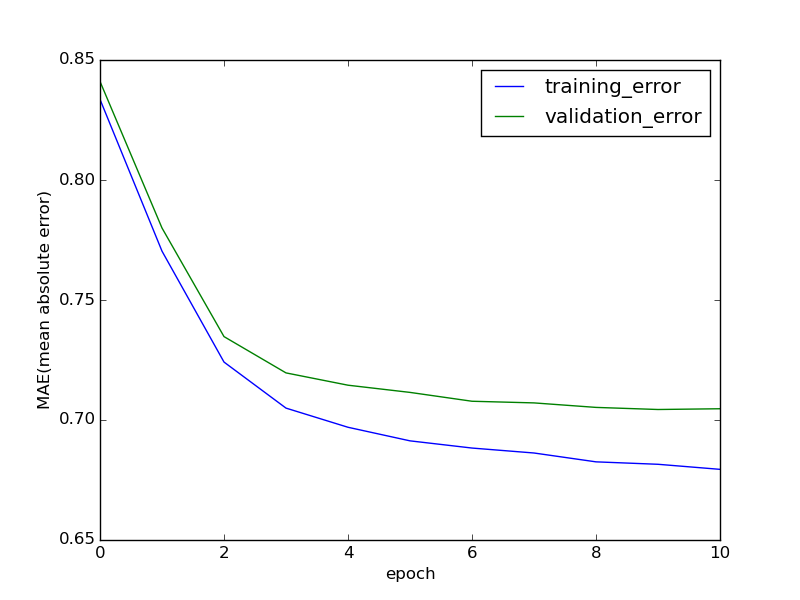
\includegraphics[width=\textwidth]{movieLens100K}
		\caption{MovieLens 100K}
		\label{fig:movieLens100K}
	\end{subfigure}
	\begin{subfigure}{0.4\textwidth}
		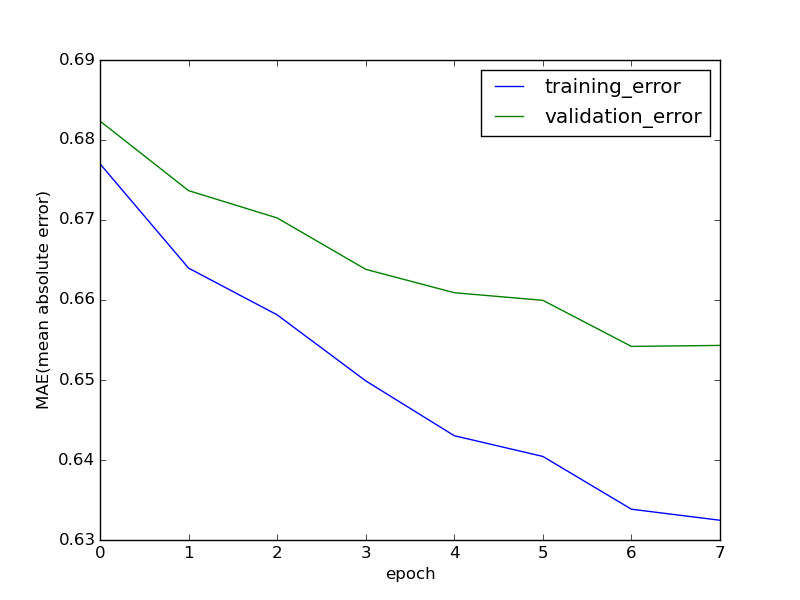
\includegraphics[width=\textwidth]{movieLens1M}
		\caption{MovieLens 1M}
		\label{fig:movieLens1M}
	\end{subfigure}
	\caption{Two example learning processes on different datasets:
	The estimator stops learning when validation errors start increasing at 
	the last epochs. 
	The testing errors are 0.711 for MovieLens 100K and 0.655 for MovieLens 1M.}
	\label{fig:trainnig}
\end{figure}

\subsection{Experiment results}
In our experiments, the neural recommender model achieves 7\% to 17\% lower 
prediction errors than the best solutions provided by collaborative filtering 
and its variants benchmarked in \cite{hwang2016efficient} and 
\cite{polatidis2016multi}, shown in \autoref{tab:accuracy}.
The neural recommender model is also very robust against 
parameter changes, shown in \autoref{tab:robust}.
\begin{table}[h]
	\centering
	\caption{The comparison of prediction errors (measured by MAE):
		the neural recommender model (NR) achieves 7\% to 17\% error reduction 
		from the baseline - collaborative filtering (CF).}
	\begin{tabularx}{0.5\textwidth}{ |X|c|c|c| }  \hline
		\textbf{Dataset} & \textbf{CF} & \textbf{NR} & \textbf{reduction} 
		\\ \hline
		MovieLens 100K & 0.74 & 0.69 & 7\% \\ \hline
		MovieLens 1M & 0.79 & 0.65 & 17\% \\ \hline
	\end{tabularx}
	\label{tab:accuracy}
\end{table}
\begin{table*}[h]
	\centering
	\caption{High robustness of the estimator against parameter changes:
		The estimator maintains testing errors in range [0.69, 0.72] for a wide 
		range of parameters. These experiments are on MovieLens 100K dataset.}
	\begin{tabularx}{\textwidth}{ |X|c|c|c|c| } \hline
		 \textbf{Learning rate} & \textbf{Keep probability} & \textbf{Layer 
		 size} & \textbf{Number of hidden layers} & \textbf{Testing error} \\ 
		 \hline
		 0.05 & 0.6 & 64 & 2 & 0.7143 \\ \hline
		 0.01 & 0.6 & 64 & 2 & 0.7109 \\ \hline
		 0.1 & 0.6 & 64 & 2 & 0.7114 \\ \hline
		 0.1 & 0.8 & 64 & 2 & 0.7058 \\ \hline
		 0.1 & 0.9 & 64 & 2 & 0.6925 \\ \hline
		 0.1 & 0.9 & 32 & 2 & 0.6965 \\ \hline
		 0.1 & 0.9 & 128 & 2 & 0.7026 \\ \hline
		 0.1 & 0.9 & 32 & 1 & 0.7032 \\ \hline
		 0.1 & 0.9 & 32 & 4 & 0.7008 \\ \hline
	\end{tabularx}
	\label{tab:robust}
\end{table*}

\subsection{Computing resources}
We ran our experiments on a Dell Optiplex 780 machine with following 
configurations:
\begin{itemize}
	\item Python implementation: CPython 3.4
	\item OS: Ubuntu 15.10 64-bit
	\item Processor: Intel Core 2 Duo CPU E8400 @ 3GHz
	\item Memory: 4GB
\end{itemize}
Each run (learning and prediction) takes around 1 to 8 minutes, 4 to 16 epochs, 
depending on the dataset and parameters.
Our implementation exploits thread level parallelism, but we have not explored 
data level parallelism (i.e., GPU) or process level parallelism (e.g., remote 
procedure call).

\section{Strengths}

\subsection{Node-centered learning}
The node mapping technique takes a node-centered approach as the estimator 
extracts knowledge of nodes from links.
In a social network, this leverages the fact that who a user contacts and what 
movies a user likes tell us what kind of person he is and help us predict his 
behavior.
It effectively learns complex and unobservable user attributes (node 
attributes) from simple and observable user activities (link attributes). 
\autoref{tab:nodesVSlinks} compares nodes and links with respect to their 
complexity and observability.
\begin{table}[h]
	\centering
	\caption{A comparison of nodes and links with respect to their complexity 
		and attribute observability in a social network:
		Links tend to have low complexity and high observability while nodes 
		are the opposite.
		For example, it is easy to observe simple user activities like sending 
		messages to other users and giving ratings to movies,
		but it is hard to observe complex user attributes like personality, 
		style or taste in movies.}
	\begin{tabularx}{0.5\textwidth}{ |X|c|c| } \hline
		\textbf{Aspect} & \textbf{Node} & \textbf{Link} \\ \hline
		complexity & high & low \\ \hline
		observability & low & high \\ \hline
		example & user & rates, likes, messages \\ \hline
	\end{tabularx}
	\label{tab:nodesVSlinks}
\end{table}

\subsection{Online learning}
The learning is online when the estimator learns for only one epoch. In 
this case, its prediction accuracy will be lower, but it naturally handles 
streaming graphs:
\begin{itemize}
	\item it can handle a new node by inserting a new vector into the mapping 
	table
	\item it does not need to handle new links as it uses every link once and 
	then discards the link
	\item it does not construct the graph or perform any complex graph 
	operations like neighbor nodes lookup
\end{itemize}
We have not explored more sophisticated techniques for streaming graphs like 
caching a finite set of new links/nodes and learning for multiple epochs on 
that set.

\section{Future work}
We are interested in using this node mapping technique to provide solutions to 
more prediction tasks in graph applications. Many of these tasks fall into the 
category of recommendation in a social network, e.g., recommending friends or 
posts to users.
Specifically, we consider to study how to use this technique to handle the 
following scenarios:
\begin{itemize}
	\item handle graphs with arbitrary topologies: e.g., given a social 
	network where users send messages each other, the estimator should 
	predict the amount of messages from one user to another
	\item handle links with string attributes: e.g., given a text message from 
	user A to user B (a link from A to B with a string attribute), the 
	estimator should extract knowledge of the users from the message content
	\item handle links with logical implications: e.g., given a user has 
	written an article (a link from user to article with a write attribute), 
	the estimator should extract knowledge of the user and the article from 
	this activity
	\item handle nodes with rich attributes: e.g., given an article (a node 
	with a string attribute) or an image (a node with an image attribute), the 
	estimator should extract knowledge of the node from the article or image 
	content and integrate this knowledge to that extracted from links
\end{itemize}
We have a Python implementation under MIT license hosted on Github.
%\footnote{https://github.com/yuchenhou/elephant}
The main machine learning packages are TensorFlow \cite{abadi2016tensorflow}.
%\footnote{https://github.com/tensorflow/tensorflow}
Do not hesitate to contact us if you are interested in our work.

\section{Conclusions}
Node mapping is an effective technique to predict link attributes in a graph 
using a neural net model.
The estimator learns both to map each node to a vector, and to predict 
the target link attribute using these vectors.
It provides a recommender systems solution that achieves better rating 
prediction accuracy than collaborative filtering and many of its variants.
For recommendation tasks in social networks, this technique realizes the idea 
of understanding complex users from their simple activities, and using that 
understanding to predict their future activities.

%\section*{Acknowledgements}
%This material is based on work supported by the National Science Foundation 
%under Grant No. 1318913.

\bibliographystyle{plain}
\bibliography{references}

\end{document}
